\documentclass[border=10pt]{standalone}

\usepackage{tikz}
\usepackage{tikzsymbols}
\usetikzlibrary{calc,patterns,shapes.geometric}

\def\centerarc[#1](#2)(#3:#4:#5){\draw[#1] ($(#2)+({#5*cos(#3)},{#5*sin(#3)})$) arc (#3:#4:#5);}

\begin{document}
	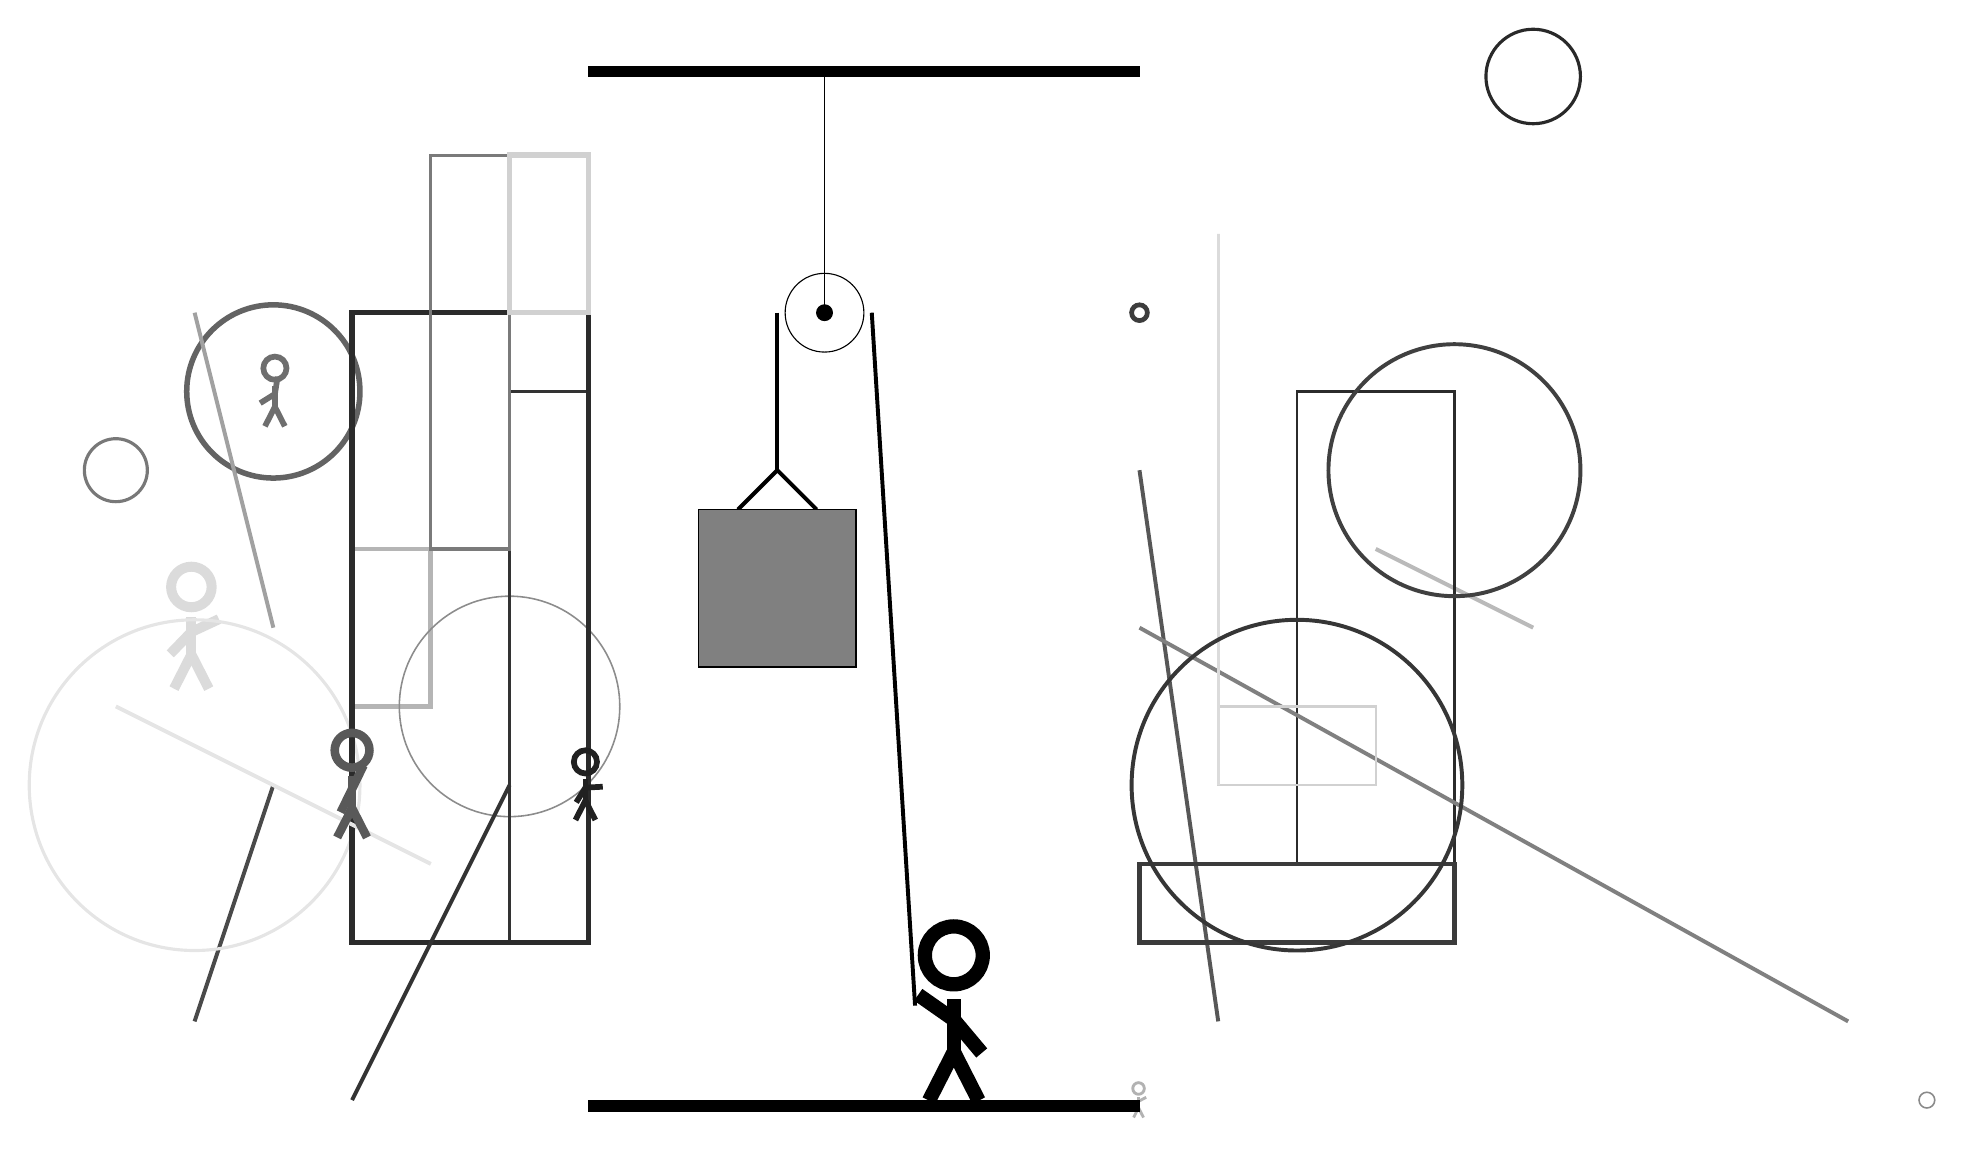
\begin{tikzpicture}
		%%%%% START %%%%%
		
		\draw[fill=black] (-2, 10) rectangle (5, 10.125);
		
		\draw [line width=0.7mm, color=black!61](-6, 6) circle (1.1);
		
		\draw[line width=0.5mm, color=black!71](-6, 1) -- (-7, -2);
		\draw[line width=0.5mm, color=black!66](6, -2) -- (5, 5);
		\draw[line width=0.5mm, color=black!27](10, 3) -- (8, 4);
		\node[line width=0.2mm, color=black!14] at (-7, 3) {\Strichmaxerl[7][46][25]};
		\draw[line width=0.6mm, color=black!29] (-4, 2) rectangle (-5, 4);
		\draw [line width=0.2mm, color=black!46](15, -3) circle (0.1);
		\draw [line width=0.2mm, color=black!45](-3, 2) circle (1.4);
		\draw[line width=0.5mm, color=black!37](-6, 3) -- (-7, 7);
		
		\draw[line width=0.4mm, color=black!80] (-3, -1) rectangle (-2, 6);
		\draw[line width=0.3mm, color=black!83] (7, 0) rectangle (9, 6);
		\draw [line width=0.4mm, color=black!10](-7, 1) circle (2.1);
		\draw[line width=0.5mm, color=black!50](5, 3) -- (14, -2);
		
		\draw[line width=0.7mm, color=black!83] (-2, -1) rectangle (-5, 7);
		\draw[line width=0.6mm, color=black!77] (5, 0) rectangle (9, -1);
		\draw[line width=0.3mm, color=black!18] (6, 1) rectangle (8, 2);
		
		\draw[line width=0.4mm, color=black!14] (6, 1) rectangle (6, 8);
		\node[line width=0.3mm, color=black!57] at (-6, 6) {\Strichmaxerl[4][32][81]};
		\draw[line width=0.4mm, color=black!52] (-3, 4) rectangle (-4, 9);
		\draw[line width=0.5mm, color=black!80](-3, 1) -- (-5, -3);
		\draw [line width=0.5mm, color=black!75](9, 5) circle (1.6);
		
		\draw [line width=0.4mm, color=black!53](-8, 5) circle (0.4);
		\draw[line width=0.7mm, color=black!18] (-2, 9) rectangle (-3, 7);
		\draw [line width=0.5mm, color=black!79](7, 1) circle (2.1);
		\draw[line width=0.5mm, color=black!10](-4, 0) -- (-8, 2);
		
		\node[line width=0.6mm, color=black!30] at (5, -3) {\Strichmaxerl[2][59][28]};
		\draw [line width=0.6mm, color=black!76](5, 7) circle (0.1);
		\draw [line width=0.4mm, color=black!84](10, 10) circle (0.6);
		
		\node[line width=0.7mm, color=black!65] at (-5, 1) {\Strichmaxerl[6][64][64]};
		\node[line width=0.2mm, color=black!87] at (-2, 1) {\Strichmaxerl[4][58][3]};
		
		\draw (1, 7) circle (0.5);
		\draw[fill=black] (1, 7) circle (0.1);
		\draw (1, 10) -- (1, 7);
		
		\draw[line width=0.5mm] (-0.1, 4.5) -- (0.4, 5.0) -- (0.9, 4.5);
		\draw[fill=black!50] (-0.6, 4.5) rectangle (1.4, 2.5);
		
		\draw[line width=0.5mm] (0.4, 7) -- (0.4, 5.0);
		\centerarc[line width=0.5mm](1, 7)(0:180:0.6);
		\draw[line width=0.5mm](1.6, 7) -- (2.15, -1.8);
		
		\node at (2.6, -1.9) {\Strichmaxerl[10][-35][-50]};
		
		\draw[fill=black] (-2, -3) rectangle (5, -3.15);
		
		%%%%% END %%%%%
	\end{tikzpicture}
\end{document}